\begin{exercice}
Simplifier les fractions suivantes : 
\begin{multicols}{2}
\begin{enumerate}
\item $$\frac{14{{b}^{4}}x\cdot 5ay}{15{{a}^{2}}x\cdot 7{{b}^{3}}y}$$
\item $$\frac{axy-bxy}{ab-{{b}^{2}}}$$
\item $$\frac{a-3}{2{{a}^{2}}-18}$$
\item $$\frac{9{{a}^{5}}-16a}{6{{a}^{2}}{{b}^{2}}-8{{b}^{2}}}$$
\item $$\frac{{{a}^{3}}+{{b}^{3}}}{{{(a-b)}^{2}}+ab}$$
\item $$\frac{4{{(x+y)}^{2}}}{3({{x}^{2}}-{{y}^{2}})}$$
\item $$\frac{{{x}^{2}}-4x+4}{{{x}^{2}}-4}$$
\item $$\frac{8{{a}^{3}}+1}{64{{a}^{6}}-1}$$
\item $$\frac{25{{x}^{2}}+20ax+4{{a}^{2}}}{2(25a{{x}^{3}}-4{{a}^{3}}x)}$$
\item $$\frac{12a{{x}^{2}}+3ax}{8{{x}^{2}}+22x+5}$$
\item $$\frac{{{x}^{2}}-7x-8}{{{x}^{3}}+3{{x}^{2}}+2x}$$
\item $$\frac{8{{x}^{2}}+22x-6}{4{{x}^{2}}+27x-7}$$
\item $$\frac{2{{x}^{2}}-9x+7}{12{{x}^{2}}-21x+9}$$
\item $$\frac{40{{x}^{3}}-5}{12{{x}^{2}}+6x+3}$$
\item $$\frac{{{(a+b)}^{2}}({{a}^{3}}-{{b}^{3}})}{{{({{a}^{2}}-{{b}^{2}})}^{2}}}$$
\item $$\frac{{{x}^{3}}-{{x}^{2}}-4x+4}{{{x}^{2}}-3x+2}$$
\item $$\frac{2{{x}^{3}}+5{{x}^{2}}+4x+1}{{{x}^{3}}+3{{x}^{2}}+3x+1}$$
\item $$\frac{{{x}^{3}}-9{{x}^{2}}+11x+21}{{{x}^{4}}-{{x}^{3}}-4{{x}^{2}}-5x-3}$$
\item $$\frac{{{x}^{4}}-2{{x}^{2}}+1}{3{{x}^{5}}-10{{x}^{3}}+15x-8}$$
\item $$\frac{1+{{x}^{3}}}{1+2x+2{{x}^{2}}+{{x}^{3}}}$$
\item $$\frac{2{{x}^{3}}-7{{x}^{2}}+2x+3}{2{{x}^{3}}-9{{x}^{2}}+10x-3}$$
\end{enumerate}
\end{multicols}
\end{exercice}

\begin{exercice}
Effectuer les opérations suivantes et simplifier :
\begin{multicols}{2}
\begin{enumerate}
\item $$\frac{x+3}{3}+\frac{x-2}{2}$$
\item $$\frac{x+3}{3}-\frac{x-2}{2}$$
\item $$\frac{a+b}{a}+\frac{a+b}{b}$$
\item $$\frac{a+b}{a}-\frac{b-a}{b}$$
\item $$\frac{3}{x-6}-\frac{1}{x-2}$$
\item $$\frac{2{{x}^{2}}}{{{x}^{2}}-{{y}^{2}}}-\frac{2{{x}^{2}}}{{{x}^{2}}+xy}$$
\item $$\frac{{{x}^{2}}}{x-{{x}^{3}}}-\frac{x}{1+{{x}^{2}}}$$
\item $$\frac{2}{2-x}-\frac{x}{x-2}$$
\item $$\frac{5}{{{a}^{2}}-1}+\frac{5}{1-a}$$
\item $$\frac{a}{a-b}+\frac{b}{b-a}$$
\item $$\frac{3}{1-{{x}^{2}}}-\frac{2}{x-1}$$
\item $$\frac{{{y}^{2}}}{{{x}^{3}}-{{y}^{3}}}+\frac{{{x}^{3}}{{y}^{2}}}{{{y}^{6}}-{{x}^{6}}}$$
\item $${{a}^{2}}-\frac{{{x}^{3}}}{a}$$
\item $$1-\frac{a-b}{a+b}$$
\item $$x-\frac{{{x}^{2}}}{a+x}$$
\item \item $$x+y+\frac{{{x}^{2}}-{{y}^{2}}}{x-y}$$
\item $$x+2-\frac{{{x}^{2}}-2x+4}{x+2}$$
\item $$1+x+{{x}^{2}}+\frac{{{x}^{3}}}{1-x}$$
\item $$\frac{a+3}{a+4}-\frac{a+1}{a+2}$$
\item $$\frac{x+a}{a-x}-\frac{x-a}{a+x}$$
\item $$\frac{a}{x-a}-\frac{{{a}^{2}}}{{{x}^{2}}-{{a}^{2}}}$$
\item $$\frac{3}{x-3}+\frac{2x}{{{x}^{2}}-9}$$
\item $$\frac{x+a}{x-2a}-\frac{{{x}^{2}}+2{{a}^{2}}}{{{x}^{2}}-4{{a}^{2}}}$$
\item $$1-2x+{{x}^{2}}+\frac{1-{{x}^{4}}}{1+2x+{{x}^{2}}}$$
\item $$\frac{5x-1}{8}-\frac{3x-2}{7}+\frac{x-5}{4}$$
\item $$\frac{x-2y}{xy}+\frac{3y-a}{ay}-\frac{3x-2a}{ax}$$
\item $$\frac{a-x}{x}+\frac{a+x}{a}-\frac{{{a}^{2}}-{{x}^{2}}}{2ax}$$
\item $$\frac{2}{xy}-\frac{3{{y}^{2}}-{{x}^{2}}}{x{{y}^{3}}}+\frac{xy+{{y}^{2}}}{{{x}^{2}}{{y}^{2}}}$$
\item $$\frac{1}{x+y}-\frac{1}{x-y}+\frac{2x}{{{x}^{2}}-{{y}^{2}}}$$
\item $$\frac{12}{9-{{a}^{2}}}-\frac{2}{3+a}-\frac{1}{3-a}$$
\item $$\frac{a}{a+b}+\frac{b}{a-b}-\frac{2ab}{{{a}^{2}}-{{b}^{2}}}$$
\item $$\frac{{{a}^{2}}+{{b}^{2}}}{{{a}^{2}}-{{b}^{2}}}+\frac{b}{a-b}-\frac{a}{a+b}$$
\item $$\frac{a+8}{a-1}+\frac{a+4}{a+1}-\frac{2(4a+1)}{{{a}^{2}}-1}$$
\item $$\frac{{{a}^{3}}-{{b}^{3}}}{{{a}^{2}}-{{b}^{2}}}-\frac{{{a}^{2}}b+a{{b}^{2}}}{{{a}^{2}}+ab}$$
\item $$\frac{{{a}^{2}}+ab}{{{a}^{2}}-ab}-\frac{{{a}^{3}}+2{{a}^{2}}b+a{{b}^{2}}}{{{a}^{2}}b-{{b}^{3}}}$$
\item $$am(a+m)-\frac{{{a}^{4}}m+a{{m}^{4}}}{{{a}^{2}}+2am+{{m}^{2}}}$$
\end{enumerate}
\end{multicols}
\end{exercice}

\begin{exercice}
Effectuer les opérations suivantes et simplifier : 
\begin{multicols}{2}
\begin{enumerate}
\item $$\frac{a}{2(a+b)}+\frac{2{{a}^{2}}}{3{{a}^{2}}-3{{b}^{2}}}-\frac{3b}{4a-4b}$$
\item $$\frac{a+5}{a-1}-\frac{6}{{{a}^{2}}+a+1}-\frac{6({{a}^{2}}+2)}{{{a}^{3}}-1}$$
\item $$\frac{a^3+ 2a^2b+ ab^2}{a^2- b^2} + \frac{a^3+ b^3}{(a-b)^2 + 2b(a-b)}$$
\item $$2+\frac{1}{2-x}+\frac{1}{2+x}+\frac{4}{{{x}^{2}}-4}$$
\item $$\frac{3}{1+a}-\frac{2}{1-a}-\frac{5a}{{{a}^{2}}-1}$$
\item $$\frac{x-a}{x+a}+\frac{{{a}^{2}}+3ax}{{{a}^{2}}-{{x}^{2}}}+\frac{x+a}{x-a}$$
\item $$\frac{3-2x}{2x+3}-\frac{2x+3}{3-2x}+\frac{36}{4{{x}^{2}}-9}$$
\item $$\frac{a{{x}^{2}}+b}{2x-1}+\frac{2(bx+a{{x}^{2}})}{1-4{{x}^{2}}}-\frac{a{{x}^{2}}-b}{2x+1}$$
\item $$\frac{x}{{{x}^{2}}+5x+6}+\frac{15}{{{x}^{2}}+9x+14}-\frac{12}{{{x}^{2}}+10x+21}$$\end{enumerate}
\end{multicols}
\begin{enumerate} \setcounter{enumi}{9}
\item $$\frac{1}{{{x}^{2}}-3x+2}+\frac{1}{{{x}^{2}}-x-2}+\frac{2}{{{x}^{2}}-1}$$
\item $$\frac{1}{{{x}^{2}}-4x+3}+\frac{1}{{{x}^{2}}-3x+2}+\frac{1}{{{x}^{2}}-5x+6}$$
\item $$\frac{{{a}^{2}}+ac}{{{a}^{2}}c-{{c}^{3}}}-\frac{{{a}^{2}}-{{c}^{2}}}{{{a}^{2}}c+2a{{c}^{2}}+{{c}^{3}}}+\frac{2c}{{{c}^{2}}-{{a}^{2}}}-\frac{3}{a+c}$$
\item $$\frac{{{a}^{2}}-2ax+{{x}^{2}}}{2({{a}^{2}}-{{x}^{2}})}-\frac{2ax(a+x)}{(a-x)({{a}^{2}}+2ax+{{x}^{2}})}-\frac{{{x}^{2}}-{{a}^{2}}}{2{{(x-a)}^{2}}}$$
\item $$\frac{1}{(a-b)(a-c)}+\frac{1}{(b-a)(b-c)}+\frac{1}{(c-a)(c-b)}$$
\item $$\frac{b-c}{(a-b)(a-c)}-\frac{c-a}{(b-a)(b-c)}+\frac{a-b}{(c-a)(c-b)}$$
\item $$\frac{{{a}^{2}}bc}{(a-b)(a-c)}+\frac{a{{b}^{2}}c}{(b-a)(b-c)}+\frac{ab{{c}^{2}}}{(c-a)(c-b)}$$ 
\end{enumerate}
\end{exercice}

\begin{exercice}
Effectuer les multiplications suivantes et simplifier : 
\begin{multicols}{2}
\begin{enumerate}
\item $$\frac{a}{6b}\cdot \frac{3b}{4}\cdot \frac{2b}{5}$$
\item $$\left( -\frac{7a}{10} \right)\cdot \frac{5a}{6}\cdot \frac{4{{x}^{2}}}{21a}$$
\item $$\left( -\frac{a}{2x} \right)\cdot \frac{8x}{9}\cdot \left( -\frac{6a}{7x} \right)$$
\item $$\left( -3{{a}^{2}} \right)\cdot \left( -\frac{11a}{15x} \right)\cdot \left( -\frac{x}{22} \right)$$
\item $$\frac{4{{x}^{2}}-6xy}{5x}\cdot \frac{10x}{6x-9y}$$
\item $$\frac{8x-2y}{x+y}\cdot \frac{2x-8y}{4x-y}$$
\item $$\frac{4+2a}{6-3a}\cdot \frac{3{{(a-2)}^{2}}}{2{{(a+2)}^{2}}}$$
\item $$\frac{6a+{{a}^{2}}}{6-a}\cdot \frac{{{a}^{2}}-36}{a}$$
\item $$\frac{{{x}^{4}}+{{x}^{2}}-2}{{{x}^{2}}+3x+2}\cdot \frac{x+1}{{{x}^{2}}-1}$$
\item $$\frac{2{{x}^{2}}-3x-9}{{{x}^{2}}+5x+4}\cdot \frac{x+4}{2x+3}$$
\item $$\frac{{{a}^{2}}{{x}^{2}}}{{{y}^{2}}}\cdot \frac{xy}{a(x+y)}\cdot \frac{{{x}^{2}}-{{y}^{2}}}{axy}$$
\item $$\frac{a+x}{{{(m+n)}^{3}}}\cdot \frac{{{x}^{2}}-{{y}^{2}}}{12}\cdot \frac{{{(m+n)}^{2}}}{m-n}\cdot \frac{6({{m}^{2}}-{{n}^{2}})}{x+y}$$
\item $$\frac{ab-3a}{4b-5}\cdot \frac{20b-25}{ac+2a}\cdot \frac{2b+bc}{a-5}\cdot \frac{2(5a-{{a}^{2}})}{4c}$$
\item $$\frac{{{x}^{3}}+{{y}^{3}}}{{{x}^{4}}-{{y}^{4}}}\cdot \frac{{{x}^{2}}y+{{y}^{3}}}{{{x}^{4}}+{{x}^{2}}{{y}^{2}}+{{y}^{4}}}\cdot \frac{{{x}^{2}}+xy+{{y}^{2}}}{x+y}$$
\item $$\frac{6{{x}^{2}}+5xy-6{{y}^{2}}}{3{{x}^{2}}-8xy-3{{y}^{2}}}\cdot \frac{3{{x}^{2}}-11xy+6{{y}^{2}}}{6{{x}^{2}}+11xy+3{{y}^{2}}}\cdot \frac{9{{x}^{2}}+9xy+2{{y}^{2}}}{9{{x}^{2}}-12xy+4{{y}^{2}}}$$
\item $$\left( 1-x+\frac{4+{{x}^{2}}}{1+x} \right)\cdot (1-{{x}^{2}})$$
\item $$\left( 1-x-\frac{2-{{x}^{2}}}{1+x} \right)\cdot (1-{{x}^{2}})$$
\item $$\left( \frac{1+x}{1-x}-\frac{1-x}{1+x} \right)\cdot \left( \frac{3}{4x}+\frac{x}{4}-x \right)$$
\item $$\left( \frac{1}{x-y}-\frac{1}{x+y} \right)\cdot \frac{{{x}^{2}}-{{y}^{2}}}{2y}$$
\item $$\left( {{x}^{2}}-xy+{{y}^{2}}-\frac{2{{y}^{3}}}{x+y} \right)\cdot \frac{x+y}{x-y}$$
\item $$\left( x+2a-\frac{{{a}^{2}}}{2x+3a} \right)\cdot \left( 2x-a-\frac{2{{a}^{2}}}{x+a} \right)$$
\item $$(x+2)\cdot \left( 1+\frac{6x+12}{{{x}^{2}}-x-6} \right)\cdot \left( 1-\frac{5x+5}{{{x}^{2}}+3x+2} \right)$$ 
\end{enumerate}
\end{multicols}
\end{exercice}

\begin{exercice}
Effectuer les divisions suivantes et simplifier : 
\begin{multicols}{2}
\begin{enumerate}
\item $$(x+y)\div \frac{x+y}{x-y}$$
\item $$({{a}^{2}}-{{b}^{2}})\div \frac{a+b}{a-b}$$
\item $$\frac{({{a}^{2}}-4)}{b+3}\div \frac{a+2}{{{b}^{2}}-9}$$
\item $$\frac{4{{x}^{2}}-9{{a}^{4}}}{ab-{{a}^{2}}}\div \frac{2x-3{{a}^{2}}}{{{a}^{3}}b-{{a}^{4}}}$$
\item $$\frac{{{(a+b)}^{2}}}{x-y}\div \frac{{{a}^{2}}-{{b}^{2}}}{{{x}^{2}}-{{y}^{2}}}$$
\item $$\frac{20x-25}{3b-4}\div \frac{4{{a}^{2}}x-5{{a}^{2}}}{9{{b}^{2}}-16}$$
\item $$\left( \frac{{{a}^{2}}}{{{x}^{2}}}-\frac{{{x}^{2}}}{{{a}^{2}}} \right)\div \left( \frac{a}{x}+\frac{x}{a} \right)$$
\item $$\left( \frac{1}{{{a}^{2}}}-\frac{1}{{{x}^{2}}} \right)\div \left( \frac{1}{x}-\frac{1}{a} \right)$$
\item $$\left( {{a}^{4}}-\frac{1}{{{a}^{2}}} \right)\div \left( {{a}^{2}}+\frac{1}{a} \right)$$
\item $$\left( 1-\frac{1}{{{x}^{2}}} \right)\div \left( \frac{a}{{{x}^{2}}}+\frac{a}{x} \right)$$
\item $$\left( 1+\frac{{{a}^{3}}}{{{x}^{3}}} \right)\div \left( \frac{1}{{{x}^{2}}}+\frac{a}{{{x}^{3}}} \right)$$
\item $$\left( 1+\frac{x-a}{x+a} \right)\div \left( \frac{x+a}{x-a}-1 \right)$$
\item $$\left( \frac{1}{x}-\frac{2}{{{x}^{2}}}-\frac{3}{{{x}^{3}}} \right)\div \left( \frac{1}{{{x}^{2}}}-1 \right)$$
\item $$\left( 2{{x}^{2}}-x-6 \right)\div \left( \frac{4}{{{x}^{2}}}-1 \right)$$
\item $$\frac{2}{1-{{x}^{2}}}\div \left( \frac{1}{1-x}-\frac{1}{1+x} \right)$$
\item $$\left( \frac{{{a}^{3}}-{{b}^{3}}}{a-b}-\frac{{{a}^{3}}+{{b}^{3}}}{a+b} \right)\div \frac{4ab}{{{a}^{2}}-{{b}^{2}}}$$ 
\end{enumerate}
\end{multicols}
\end{exercice}

\begin{exercice}

Calcul des proportions
 
\begin{enumerate}
\item Application en économie
\begin{enumerate}
\item Le pourcentage : un rabais de $20 \%$

\begin{tabular}{llllll}
Rabais & 20  &     & 4 &    & 840 \\
Prix   & 100 & 200 &   & 10 &    
\end{tabular}

\item Le taux de change : 1 \euro{} = Fr. 1.17 (le 11.07.2011)

\begin{tabular}{llllll}
\euro{}   & 1    & 2 &      & 250.50 &    \\
Fr. & 1.17 &   & 2.50 &        & 48
\end{tabular}
\item Le salaire d’un vendeur en fonction du chiffre d’affaire : $2 \%$ de commission

\begin{tabular}{llllll}
Ventes  & 10'000.00 & 50'000.00 &          & 1'000.00 &          \\
Salaire & 200.00    &           & 4'000.00 &          & 5'555.00
\end{tabular}

\item Le taux d’intérêt d’un compte épargne : $1.25 \%$ par année

\begin{tabular}{llllll}
Montant  & 100.00 & 12'500.00 &        & 151'000.00 &          \\
Intérêts & 1.25   &           & 480.00 &            & 1'234.56
\end{tabular}
\end{enumerate}
 
\item Application en politique

Les votations : en février 2011, lors de la votation pour l’initiative «pour la protection face à la violence des armes», plus de 1.395 million de personnes ont glissé un «non» dans l'urne, plus de 1.083 million un «oui». 
Quelle est la proportion de « oui » ? Quelle est la proportion de « non » ?

\item Application en géographie

\'Echelle : selon « Google Earth », il y a 821,10 mètres entre l’école ECCG de Martigny et la tour de la Bâtiaz. Sur la carte nationale 1325 au 1:25'000, indiquer la distance correspondante en centimètres.
L'évolution démographique de la Suisse : entre 2008 et 2009, l'émigration passe de 86'100 à 86'000, soit une légère baisse de ? $\%$. Les immigrations diminuent également en passant de 184'300 en 2008 à 160'600 en 2009 : soit - ?$\%$. 

\item Application en Histoire

Les morts de la Seconde Guerre mondiale

\begin{tabular}{llllll}
Pays        & \begin{tabular}[c]{@{}l@{}}Pertes\\   militaires\end{tabular} & \begin{tabular}[c]{@{}l@{}}Pertes\\   civiles\end{tabular} & \begin{tabular}[c]{@{}l@{}}Pertes\\   totales\end{tabular} & \begin{tabular}[c]{@{}l@{}}Population\\   totale d'avant-guerre\end{tabular} & \begin{tabular}[c]{@{}l@{}}Pertes\\   en\\   \%\end{tabular} \\
Pologne     & 120'000                                                       & 5'300'000                                                  & 5'420'000                                                  & 36'133'000                                                                   & ?                                                            \\
Yougoslavie & 300'000                                                       & 1'200'000                                                  & 1'500'000                                                  & ?                                                                            & 10.00\%                                                      \\
Allemagne   & 4'000'000                                                     & 3'000'000                                                  & 7'000'000                                                  & ?                                                                            & 12.00\%                                                      \\
Japon       & 2'700'000                                                     & 300'000                                                    & 3'000'000                                                  & 75'000'000                                                                   & ?                                                            \\
Italie      & 300'000                                                       & 100'000                                                    & 400'000                                                    & 40'000'000                                                                   & ?                                                            \\
France      & 250'000                                                       & 350'000                                                    & 600'000                                                    & ?                                                                            & 1.50\%                                                       \\
Royaume-Uni & 326'000                                                       & 62'000                                                     & 388'000                                                    & ?                                                                            & 0.80\%                                                       \\
États-Unis  & 300'000                                                       & -                                                          & 300'000                                                    & 150'000'000                                                                  & ?                                                           
\end{tabular}
D'après Marc NOUSCHI, Bilan de la Seconde Guerre mondiale, Le Seuil, 1996.

\item Application en sociologie

Quelle est la proportion de filles dans ta classe ? Et de garçons ?
Si le taux de réussite est de 75 %, combien d’élèves devraient réussir ?
Combien de filles réussiraient ? Et de garçons ?
 
\item Application en biologie

Qu’est-ce qui est plus grand : un virus (type grippe) ou une bactérie (type bacille) ?

 
 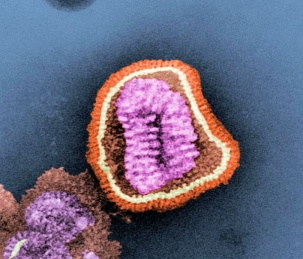
\includegraphics{fractions/virus.png}
Figure 1 : virus de la grippe au microscope électronique (en fausses couleurs)

 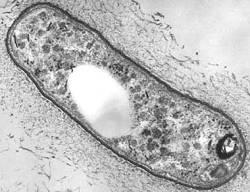
\includegraphics{fractions/bacterie.png}
Figure 2 : Une bactérie en forme de bacille
au microscope électronique

 
Sur la première photo, le virus mesure 1.5 cm et l'échelle est indiquée : 8 mm pour 25 nm
Sur la seconde image, la bactérie mesure 3.4 cm et l'échelle est indiquée : 4.2 cm pour 2 $\mu m$.
Rappel : 1 mm = 1 millimètre = 1'000 $\mu m$ = 1'000 micromètres = 1'000'000 nm = 1'000'000 nanomètres 
\end{enumerate}

\end{exercice}